\setcounter{footnote}{0}
\setcounter{figure}{0}
\setcounter{table}{0}
\chapter*{Implicações dos experimentos sobre atitudes implícitas para uma análise experimental feminista do comportamento}
\addtocontents{toc}{\vspace{\normalbaselineskip}}
\addcontentsline{toc}{chapter}{Capítulo 5}
\addcontentsline{toc}{section}{Implicações dos experimentos sobre atitudes implícitas para uma análise experimental feminista do comportamento}
\addcontentsline{toc}{subsection}{\textbf{Autoras:} \textit{ Madeleine Reinert Marcelino \& Ana Arantes}}
\begin{flushright}
\begin{small}
    Madeleine Reinert Marcelino\\
    Ana Arantes\footnote{As autoras agradecem a contribuição preciosa de Júlia Castro Freitas na indicação de bibliografia, esclarecimento de procedimentos e debate das ideias que resultaram neste capítulo.}\\
\end{small}
\vspace{1cm}
\end{flushright}

O conceito de atitude é descrito de maneiras variadas entre diversas disciplinas e ao longo do tempo. Psicólogos sociais entendem como atitude o conjunto de respostas afetivas generalizadas diante de determinados estímulos e contextos (Lloyd, 1994). De maneira geral, as teorias psicológicas tradicionais entendem como atitude o relato verbal de uma predisposição emocional em direção a objetos ou eventos do mundo (Guerin, 1994). Para Bem (1965), as atitudes de uma pessoa sobre um determinado contexto de estímulos seriam, em certo grau, preditivas do comportamento desse indivíduo quando confrontado com esse contexto, porém estudos posteriores demonstraram que nem sempre as atitudes relatadas são consistentes com o comportamento, ou preditivas deste (Ajzen \& Madden, 1986; Kashima, Gallois, \& McCamish, 1993; Lloyd, 1994). Para Catania (2017), o que comumente se descreve como atitudes, intenções e atribuições são respostas operantes discriminadas e verbalmente governadas, ensinadas e mantidas por práticas da comunidade verbal a que o indivíduo pertence.

Atitude é um construto geralmente aplicado como explicação para o comportamento observado depois que o indivíduo já se comportou, mas não necessariamente faz parte do conjunto de variáveis múltiplas que controlam essa resposta observada (ver também Field \& Hineline, 2008 e Hineline, 1990). Em uma interpretação analítico-comportamen\-tal, esta poderia ser uma clássica situação em que as atitudes explícitas, que podem ser analisadas como respostas operantes verbais de tato, mando ou intraverbais (Guerin, 1994), são controladas em parte pela audiência (Skinner, 1957). Uma parte significante da população universitária, por exemplo, relataria atitudes positivas diante do gênero feminino (como afirmar que deve haver igualdade de direitos entre homens e mulheres, que mulheres são tão competentes academicamente quanto homens, etc.) e atitudes negativas diante de situações de violência contra a mulher (abusos psicológicos, físicos, emocionais e/ou sexuais de mulheres, perpetrados por homens, com a função de controlar o comportamento das mulheres). Essas pessoas, provavelmente, diante da afirmação ``uma mulher vítima de estupro sempre tem parte da culpa quando está bêbada e usando roupas curtas, justas e provocantes'', emitiriam respostas verbais de repulsa e recusa, ou seja, teriam atitudes negativas diante desse contexto, como dizer que a afirmação apresentada é falsa ou machista. Os relatos verbais emitidos diante desse contexto são comportamentos verbais controlados por regras (configurando, assim, um operante intraverbal) ou, ao menos, tatos impuros\footnote{A teoria do comportamento verbal de Skinner (1957) define o operante verbal de tato como a resposta verbal sob controle de estímulos ou propriedades de estímulos não verbais do ambiente, mantida por reforçamento social generalizado. O tato impuro seria a resposta de tato que, além do controle pelo estímulo não verbal, teria também componentes de controle próprios de outros operantes verbais, como controle intraverbal (quando o tato é emitido diante de uma pergunta – estímulo antecedente verbal), ou no caso da ``mentira'', quando o tato é emitido sob condições de operação motivacional específica, controle próprio do operante verbal de mando.} selecionados e mantidos por contingências verbais específicas do grupo social universitário (Skinner, 1957). Podemos formular, por exemplo, as hipóteses de que é esperado que se rejeite comportamentos considerados machistas na comunidade verbal acadêmica e que, diante dessa audiência, relatos verbais considerados machistas são punidos e relatos considerados feministas são reforçados. Essas respostas verbais estão presentes no repertório do indivíduo ainda que outros comportamentos verbais ou não verbais denotem o contrário do que é relatado, pois, na prática, quando estão diante de situações em que agressões sexuais ocorreram, os universitários podem emitir comportamentos de culpabilização de uma vítima de estupro, como questionar com que roupas ela estava, se estava bêbada ou se ela havia ido ao local onde o estupro ocorreu de livre e espontânea vontade. Isso demonstra atitudes implícitas controladas por diferentes relações entre estímulos do ambiente, que são socialmente aprendidas.

Segundo a literatura psicológica não comportamental, medidas de atitudes explícitas requerem atenção consciente, estando assim sujeitas ao problema da desejabilidade social (Crowne \& Marlowe, 1960), enquanto medidas de atitudes implícitas eliminam esses problemas, pois não dependem da reflexão consciente, sendo espontâneas e automáticas (Fazio \& Olson, 2003). Quando pesquisadores apresentam questionários, checklists e entrevistas aos participantes de pesquisa, a medida resultante é a do relato verbal, os participantes dizem como se comportariam no futuro ou como já se comportaram no passado diante de determinados contextos de estimulação. Não necessariamente o controle sobre esse \textit{dizer} (resposta operante verbal) vem do mesmo tipo de estimulação antecedente e consequente que controlaria as respostas não verbais, automáticas e imediatas diante do contexto no qual se quer medir o comportamento atitudinal do indivíduo (ver, p. ex., Israel \& O'Leary, 1973; Israel, 1978 para uma discussão sobre a independência funcional dos repertórios verbais e não verbais). Essa discrepância resultaria, assim, em dados falsos sobre a atitude das pessoas em relação a determinados temas, já que a atitude medida pelos instrumentos explícitos não seria o mesmo comportamento que se quer prever em ambiente natural, mas o relato verbal de uma regra socialmente aprendida e mantida por uma audiência específica. Entretanto, as medidas explícitas têm dominado a literatura empírica, sendo bastante populares entre os psicólogos sociais (Gawronski \& Bodenhausen, 2006; Maio \& Haddock, 2010). 

Já a literatura de Análise do Comportamento, por sua rejeição a explicações mentalistas e internalistas para a ocorrência do comportamento, compreende o conceito de atitude a partir das variáveis ambientais responsáveis pelo aprendizado e manutenção dos repertórios comportamentais considerados atitudinais. Um dos argumentos a favor de adotarmos uma abordagem analítico-comportamental do conceito de atitude é porque o construto apresentado na literatura psicológica não comportamental acaba sendo circular (a pessoa se comporta de tal forma diante do objeto porque tem uma atitude sobre ele e nós só sabemos que a pessoa tem uma atitude sobre o objeto porque a pessoa se comporta de tal forma diante dele). Note que essa explicação não nos dá muitas informações sobre os eventos ambientais dos quais esse comportamento é função e muito menos nos aponta soluções para modificar esses comportamentos. Uma vez que a Análise do Comportamento é uma ciência que pode ser usada na superação de injustiças sociais derivadas de preconceitos, é importante que ela ofereça conhecimentos para explicar esses fenômenos e também que aponte caminhos para mudança (Holland, 1973).

Outras variáveis podem influenciar as medidas explícitas, de modo que elas não sejam sempre eficientes para predizer o comportamento das pessoas. Nosek, Hawkins e Frazier (2011) apontam que as medidas explícitas não são eficientes para predizer comportamentos em algumas situações, pois: a) pessoas podem ter uma reação implícita sobre determinado assunto, mas não a reportarem, pois não têm motivação para revelar (porque discordam delas ou não querem expressá-las por medo de serem punidas); b) podem ter motivação para revelar, mas não a oportunidade para tanto devido às características do instrumento; c) pode não ter habilidade para reportar, mesmo que tenham motivação e oportunidade; e, por fim, d) podem simplesmente não conseguir relatar verbalmente (ou seja, não têm o repertório de tatos correspondentes, pela definição analítico-comportamental) a relação do conteúdo implícito com seu repertório de comportamentos.

Sendo assim, ao longo das últimas duas décadas foram desenvolvidos mais de 20 tipos diferentes de testes de medidas implícitas que são usados por diversos pesquisadores para observar e medir atitudes (ver Nosek et al. 2011, para uma revisão dos instrumentos de medidas implícitas). Um estudo de Watt, Keenan, Barnes e Cairns (1991) inaugurou a área desenvolvendo um procedimento no qual os participantes de pesquisa de grupos sociais distintos em religião e nacionalidade (protestantes da Irlanda do Norte, protestantes ingleses e católicos da Irlanda do Norte) foram expostos a tarefas de \textit{matching-to-sample} (MTS, do inglês para pareamento com o modelo) em que aprendiam diferentes relações condicionais entre estímulos: as relações A-B, entre sobrenomes católicos (A) e sílabas sem sentido (B); e B-C, entre sílabas sem sentido (B) e símbolos protestantes (C). Durante a fase de testes de relações de equivalência, os participantes de origem inglesa responderam de acordo com a relação AC, combinando os nomes católicos com os símbolos protestantes. Porém, 12 dos 19 participantes da Irlanda do Norte escolheram um nome protestante na presença do símbolo protestante, sugerindo que classes de estímulos aprendidas anteriormente ao experimento, devido à experiência com contingências sociais daquele país, interferiam no estabelecimento de novas relações entre os estímulos apresentados, que eram incompatíveis com aquelas já instaladas no repertório comportamental dos participantes.

O teste de medidas implícitas mais utilizado, segundo a revisão de Nosek et al. (2011), é o \textit{Implicit Association Test} (IAT, sigla em inglês para Teste de Associação Implícita), que é um instrumento cujo objetivo é detectar o poder de associações automáticas entre as representações mentais de conceitos e objetos na memória. Ou seja, este teste exterioriza, de maneira quantitativa, os preconceitos enraizados e geralmente disfarçados durante um autorrelato, conhecidos como atitudes implícitas, utilizando como medida a latência das respostas a relações entre estímulos apresentadas em dois blocos de tarefas contrastantes. Assim, quanto maior o tempo despendido pelo participante para responder positivamente às relações apresentadas em tentativas de MTS nas tarefas consideradas pela nossa comunidade verbal como inconsistentes (por exemplo, a relação entre as palavras ``mulher'' e ``dominante''), e quanto menor o tempo despendido para realizar as tarefas consistentes (por exemplo, o tempo para responder positivamente à relação entre as palavras ``mulher'' e ``submissa''), maiores são as medidas da atitude implícita negativa em relação a mulheres no que diz respeito ao contexto de dominância (Greenwald, McGhee, \& Schwartz, 1998). A interpretação não comportamental que se faz deste fenômeno é de que processos mediacionais ou cognitivos conscientes devem estar em funcionamento quando uma pessoa é solicitada a responder de maneira imediata a uma relação inconsistente com aquelas a que ela está normalmente em contato no ambiente social, que devem evocar respostas automáticas, imediatas e, portanto, inconscientes. Durante o procedimento do IAT, feito no computador, cada palavra apresentada como estímulo, na parte de baixo da tela, deve ser associada a uma dentre duas categorias, apresentadas nos cantos superiores da tela. As respostas que denotam a consistência ou inconsistência das relações entre os estímulos (por exemplo, a palavra ``submissa'', na presença das categorias ``mulher'' e ``homem'', deve ser associada à categoria ``mulher'', denotando o viés de gênero) são emitidas pelo participante de acordo com as posições das palavras na tela do computador. As tentativas consideradas incorretas em cada bloco são seguidas de \textit{feedback} corretivo e as respostas consideradas corretas em cada bloco não são seguidas de consequências programadas. A Figura \ref{fig1} mostra um conjunto de tentativas hipotéticas de um IAT para medida de viés de gênero.

\begin{figure}[h]
    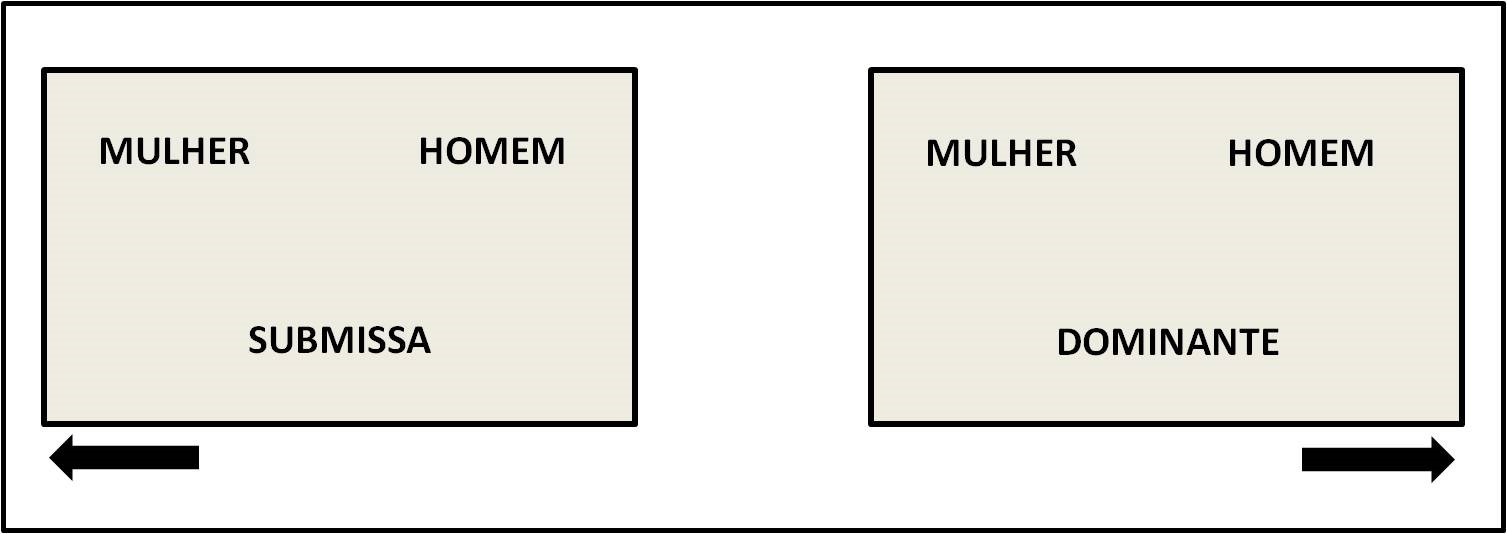
\includegraphics[width=\linewidth]{5/figura1.jpg}
    \caption{Modelo esquemático da apresentação dos estímulos em duas tentativas hipotéticas do IAT. À esquerda, a resposta considerada correta nas tentativas consistentes é apresentada pela seta preta, ou seja, na direção da categoria ``mulher''. À direita, a resposta considerada correta nas tentativas consistentes está na direção da categoria ``homem''.}
    \label{fig1}
\end{figure}

Uma alternativa ao IAT é o IRAP (da sigla em inglês para \textit{Implicit Relational Assessment Procedure} ou Procedimento de Avaliação Relacional Implícita), de Barnes-Holmes et al. (2006), que é um procedimento que utiliza as tarefas experimentais semelhantes às do IAT, porém com uma operacionalização mais aproximada da Análise do Comportamento. O IRAP é baseado em várias teorias comportamentais, como a teoria do comportamento verbal (Skinner, 1957), o paradigma de equivalência de estímulos (Sidman, 1971; 1997), e a Teoria das Molduras Relacionais (Hayes, Barnes-Holmes, \& Roche, 2001). Essas teorias comportamentais sobre o desenvolvimento do comportamento simbólico apresentam a aprendizagem, em contingências sociais, das respostas a relações entre estímulos como determinante de repertórios de responder imediato, implicados nas atitudes implícitas, durante a formação de categorias de estímulos. Assim, uma maior latência das respostas emitidas diante de uma relação entre dois estímulos (por exemplo, mulher-dominante, em comparação com homem-dominante), é interpretada como a dificuldade de modificar a função de estímulos equivalentes, como já demonstrado pela literatura (Barnes, Browne, Smeets, \& Roche, 1995; Barnes \& Keenan, 1993), especialmente\linebreak quando a nova função que se quer instalar é inconsistente ou incompatível com a função inicial do estímulo no controle das respostas do indivíduo a estímulos equivalentes\footnote{O paradigma de equivalência de estímulos proposto por Sidman (1971) é um modelo experimental da aquisição de comportamento simbólico que tem sido amplamente confirmado por dados experimentais de pesquisas tanto com humanos como com animais não-humanos (p. ex., Sidman, 1994). Sidman (1971) e Sidman e Cresson (1973), ensinaram, a jovens com atraso cognitivo severo, relações entre palavras faladas e desenhos, bem como relações entre palavras faladas e palavras impressas. Posteriormente, verificaram a emergência de relações de equivalência (o responder diante de novas relações nunca apresentadas no procedimento, de forma coerente com as relações aprendidas) entre figuras e palavras impressas, indicando que estas haviam adquirido o status de símbolos para estes participantes. Os estudos na área compreendem, tipicamente, uma fase de ensino de uma linha de base de relações condicionais entre estímulos usando-se o procedimento de MTS, seguida por uma fase de teste de relações emergentes. Os participantes que aprendem as relações ensinadas na linha de base mostram respostas coerentes diante de relações não treinadas, atestando que a função dos estímulos se tornou equivalente no controle do comportamento dos participantes.}. A função inicial do estímulo no controle do comportamento individual é aprendida em contingências sociais, dentro da cultura do indivíduo e ao longo de sua vida, sem necessariamente transferir-se para o controle do relato verbal desse indivíduo sobre seu próprio comportamento. Dentro do modelo de significado proposto pelo paradigma de equivalência de estímulos (p. ex., Sidman, 1971 e Sidman \& Cresson, 1973), as palavras e conceitos podem adquirir a mesma função no controle do comportamento a depender de relações estabelecidas dentro de uma rede, que torna os estímulos equivalentes, mesmo que não necessariamente relacionados diretamente por meio de experiência direta de condicionalidade. Por exemplo, uma pessoa pode – ao longo da sua história de aprendizagem social – nunca ter sido ensinada diretamente que ``mulheres são submissas'', mas, por meio de regras não explicitadas e de aprendizagens em contingências específicas, pode ter aprendido que ``mulheres são fracas'' e também ter aprendido a relação entre os estímulos ``pessoas fracas'' e ``submissão'', e então responder da mesma maneira à relação ``mulheres-submissão'', por transitividade das relações aprendidas anteriormente, que possuem o mesmo significado em determinados contextos do ambiente cultural. O IRAP seria, então, sensível a esse fenômeno, dado que os participantes são instruídos a responder coerentemente a determinadas relações condicionais apresentadas entre estímulos estereotipicamente relacionados dentro da cultura. Quando as relações já foram aprendidas anteriormente, e as classes de estímulos equivalentes já estão presentes no controle do repertório de respostas do indivíduo, espera-se que ele responda de maneira mais rápida durante o procedimento.

No procedimento do IRAP, a tarefa experimental é apresentada ao participante na tela do computador, e em cada tentativa são apresentados dois estímulos e duas opções de resposta (que podem ser ``correto'' e ``incorreto'', ``sim'' e ``não'', ``combina'' ou ``não combina'', etc.). O participante deve responder o mais rápido possível a uma dessas opções, diante da relação entre os dois estímulos na tela. São apresentados blocos de tentativas de treino das relações condicionais entre os estímulos e, em seguida, blocos consecutivos de tentativas de teste das relações treinadas, em que a resposta é considerada correta quando é consistente com aquela hipotetizada pelos experimentadores como produto da aprendizagem social (isto é, as respostas a relações estereotipadas do tipo ``mulher-submissa'' e ``homem-dominante''; ou ``menina-boneca'' e ``menino-carrinho''), ou blocos em que as respostas são consideradas corretas quando são inconsistentes com os estereótipos sociais (por exemplo, diante das relações ``mulher-dominante'' e ``homem-submisso''; ou ``menina-carrinho'' e ``menino-boneca''). Além disso, respostas somente são consideradas corretas se forem emitidas dentro de um período de 2s da apresentação da tentativa, caso contrário, serão consequenciadas e registradas como incorretas. Espera-se, então, que os participantes levem mais tempo para responder corretamente às tentativas de teste dos blocos inconsistentes do que às tentativas dos blocos consistentes. A Figura \ref{fig2} mostra um exemplo hipotético da configuração das tentativas apresentadas durante um procedimento de IRAP. As respostas consideradas corretas, nos blocos de tentativas de treino, são seguidas da próxima tentativa (ou seja, não há consequências específicas para acerto) e as respostas consideradas incorretas, inclusive nas tentativas em que não houve resposta dentro do tempo limite de 3s, são seguidas de consequência negativa (por exemplo, a palavra ``incorreto'' ou um X vermelho na tela do computador) e da reapresentação da mesma tentativa até que o participante emita a resposta designada como correta naquela tentativa. 

\begin{figure}[t]
    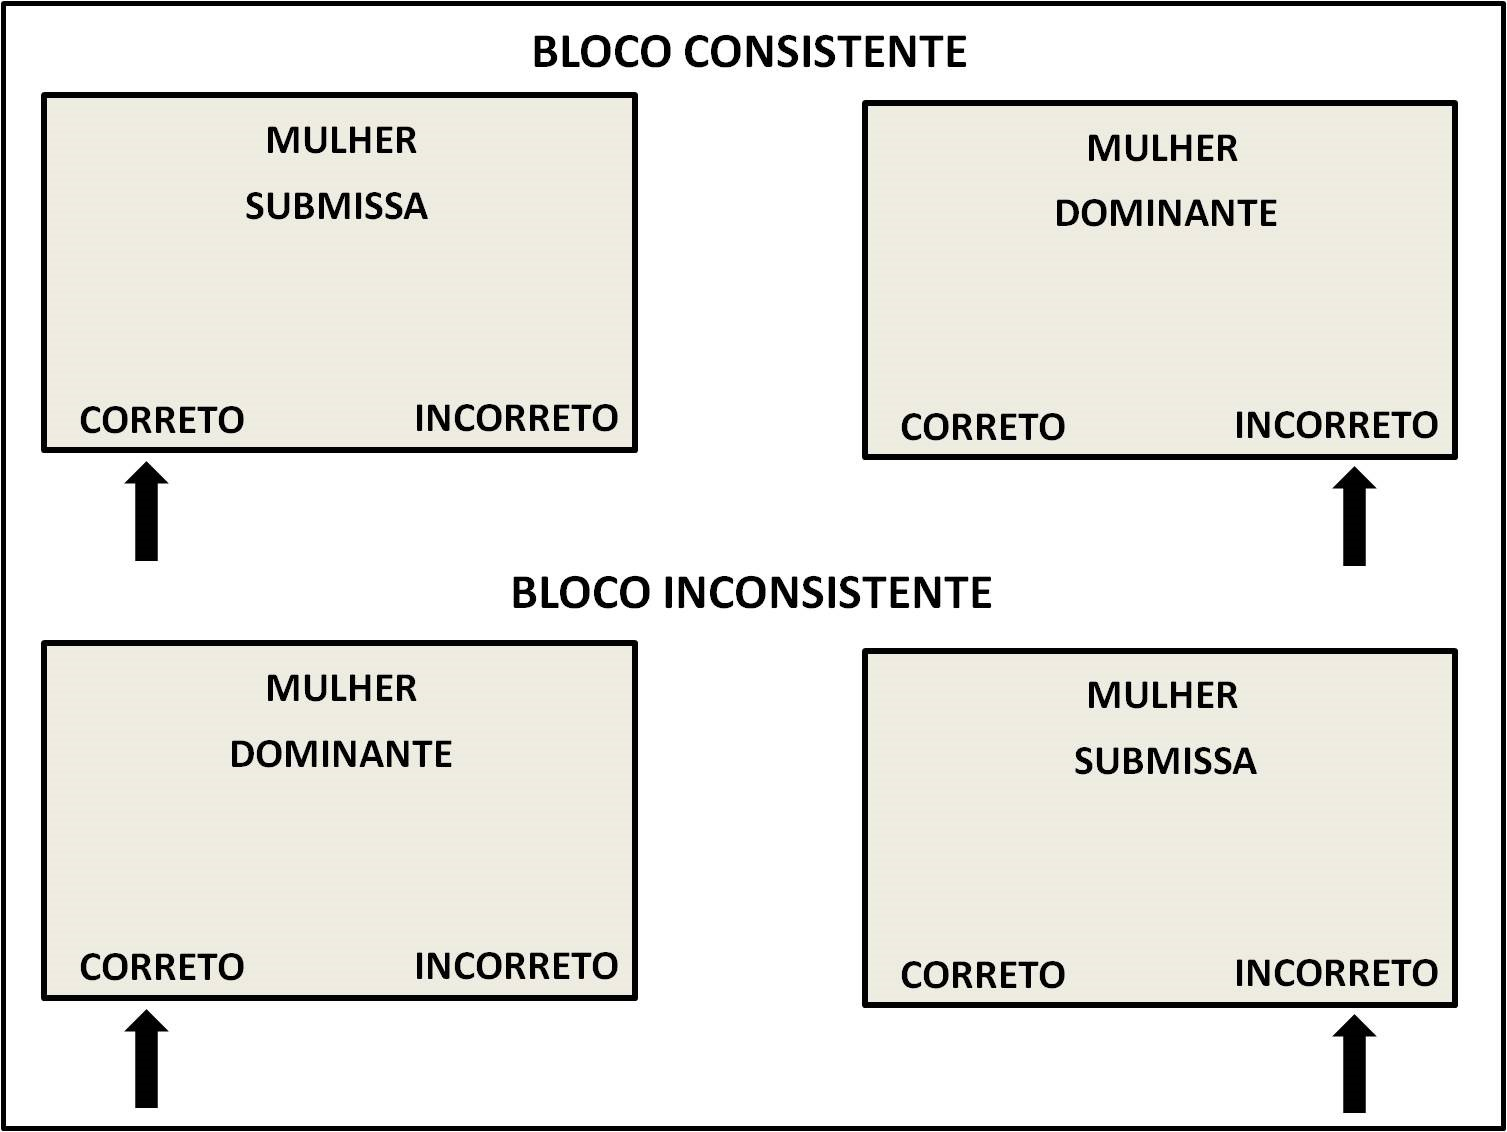
\includegraphics[width=\linewidth]{5/figura2.jpg}
    \caption{Modelo esquemático da apresentação dos estímulos nos quatro tipos de tentativas hipotéticas do IRAP. Nos blocos consistentes (acima) e nos blocos inconsistentes (abaixo) a resposta considerada correta deve ser clicar sobre a palavra que está indicada pela seta preta.}
    \label{fig2}
\end{figure}

Diversas demonstrações experimentais mostram que o IRAP pode ser usado de maneira eficiente para detectar atitudes implícitas em relação a gênero, e que os resultados do IRAP replicam o fenômeno já demonstrado com o IAT, na comparação com instrumentos de medida de atitudes explícitas, de que o relato verbal de atitudes diante de determinados contextos não é preditivo do comportamento atitudinal implícito diante do mesmo contexto. Um levantamento feito por Freitas (2017) encontrou sete estudos que usaram o IRAP para estudar estereótipos e vieses de gênero, e os resultados mostram que esse teste é sensível para detectar essas atitudes em diversos contextos. Drake et al. (2010) realizaram quatro estudos para avaliar a sensibilidade e a aplicabilidade do IRAP, buscando acrescentar avaliações de viés de raça, religião, gênero e obesidade à literatura experimental referente ao instrumento. No estudo que avaliou atitudes quanto a gênero, foram realizadas duas aplicações consecutivas do IRAP, uma em que os estímulos utilizados foram as palavras ``homem'' e ``mulher'' e profissões estereotipicamente masculinas e femininas, e outra em que os estímulos eram as palavras ``homem'' e ``mulher'' e afazeres domésticos considerados masculinos e femininos. Os resultados mostraram diferença entre as médias dos escores do IRAP para as ocupações estereotipicamente femininas, no grupo de mulheres (mulheres responderam mais rápido a relações estereotipicamente consistentes entre a palavra ``mulher'' e as ocupações femininas do que a relações inconsistentes entre esses estímulos); o mesmo aconteceu no grupo de participantes homens para as relações consistentes entre a palavra ``homem'' e as ocupações masculinas. A diferença nas outras relações não foi significativa. Esse resultado confirma a literatura sobre profissões estereotipicamente femininas, e reforça a hipótese de que o IRAP é sensível a esse tipo específico de atitude implícita no contexto de gênero.

Algumas vezes o responder atitudinal diante de contextos mistos de estímulos culturais pode mostrar viés mais forte para um tipo de estimulação do que para outro, o que nos leva a inferir que determinadas classes de estímulos equivalentes podem interagir ou até mesmo se sobrepor a outras, no controle do comportamento. Nolan, Murphy e Barnes-Holmes (2013) aplicaram o IRAP em 21 estudantes universitários para verificar atitudes em relação à obesidade, analisando se o peso corporal de uma pessoa influenciava na percepção que os participantes tinham quanto à sua inteligência. Os estímulos utilizados foram fotos de homens e mulheres antes e depois der perderem peso e adjetivos que denotam inteligência ou falta dela, por exemplo, estúpido, idiota, bobo, etc. Os resultados encontrados corroboram a hipótese de que as relações entre os estímulos ``pessoa magra'' e inteligência são muito mais automáticas (e, portanto, implícitas) do que as relações entre ``pessoas gordas'' e inteligência. Quando foram feitas análises específicas por gênero do participante, encontrou-se que os homens mostraram atitude mais favorável para a relação inteligência-magreza quando os estímulos eram fotos de homens do que quando eram fotos de mulheres, enquanto as participantes mulheres não mostraram diferenças na latência da resposta diante dos dois tipos de estímulos. Isso pode ser interpretado como uma interferência das atitudes dos participantes homens em relação ao gênero feminino no responder diante das relações entre os estímulos ``mulher'' e palavras denotativas de inteligência.

Estudos têm demonstrado que essas aprendizagens relacionais são adquiridas desde cedo no desenvolvimento dos indivíduos, provavelmente por estarem constantemente, desde antes do nascimento, em contato com as relações sociais e as práticas culturais vigentes em sua comunidade verbal. Além disso, determinados repertórios de responder relacional a configurações de estimulação do ambiente podem levar a maior ou menor grau de atitudes diante de contextos específicos. Scanlon, McEnteggart, Barnes-Holmes e Barnes-Holmes (2014) buscaram avaliar viés implícito de gênero e autoestima em crianças com desenvolvimento típico, crianças com TDAH (Transtorno do Déficit de Atenção com Hiperatividade) e crianças com dislexia. O primeiro estudo teve como participantes crianças de 8 a 11 anos, tanto com TDAH quanto com desenvolvimento típico. Os estímulos utilizados eram o nome da própria criança e um nome do outro gênero, além de três adjetivos positivos e três negativos. Os resultados mostraram que ambos os grupos apresentavam graus diferentes de atitude implícita positiva em relação a si mesmo. As crianças com desenvolvimento típico não mostraram nenhum viés em relação ao nome de outro gênero, mas as crianças com TDAH mostraram atitudes negativas quanto ao nome do gênero oposto ao delas, além das atitudes positivas quanto a si mesmas. Já o segundo estudo teve como participantes 20 crianças de nove a 14 anos, com desenvolvimento típico e com dislexia. O procedimento foi o mesmo que no primeiro estudo. Como resultado, ambos os grupos mostraram viés a favor de si mesmo tanto nos testes do tipo ``eu-positivo'' e ``eu-negativo'', e ambos os grupos não foram nem positivos nem negativos no julgamento da relação ``outro-positivo''. Contudo, as crianças de desenvolvimento típico mostraram viés contrário ao outro nas tentativas do tipo ``outro-negativo'', enquanto as que tinham dislexia mostraram viés a favor. Outro estudo com crianças foi o de Rabelo, Bortoloti e Souza (2014), que envolveu 10 crianças de sete a 10 anos. Os estímulos utilizados foram nomes femininos e masculinos e brinquedos tipicamente designados a cada um dos gêneros (bonecas e carrinhos). As crianças de ambos os sexos responderam significativamente mais rápido nas tentativas que relacionavam que bonecas eram para meninas e que bonecas não eram para meninos. As relações com os carrinhos não foram significativas. 

A história de aprendizagem de práticas culturais vigentes no grupo em que o indivíduo se insere pode ser responsável pelo viés implícito apresentado pelas pessoas ao longo da vida, de maneira inconsciente e muitas vezes difícil de detectar em situações cotidianas\footnote{Para análises mais aprofundadas das implicações dos repertórios atitudinais implícitos, veja os capítulos 02 e 04 deste livro, que fazem discussões acerca das consequências da desigualdade de gêneros.}. Farrell, Cochrane e McHugh (2015) utilizaram o IRAP com 32 adultos (sendo 16 homens e 16 mulheres), usando como estímulos as palavras homem e mulher e nomes de carreiras profissionais. Os resultados mostraram que, de maneira geral, os participantes associaram mais as carreiras de ciência, tecnologia, engenharia e matemática com homens e as carreiras artísticas com mulheres. Esse efeito foi mais proeminente nas participantes mulheres; os homens tenderam a responder de maneira mais neutra. Já Hussey et al. (2016) investigaram o fenômeno da desumanização\footnote{O fenômeno da desumanização acontece quando emitimos comportamentos que denotam que pessoas do gênero feminino têm o mesmo valor ou função que objetos. Esse tipo de repertório está implicado, por exemplo, no uso da imagem de mulheres consideradas sexualmente atrativas para vender produtos, como é feito em propagandas de cerveja.} das mulheres, também usando o IRAP. Participaram da pesquisa 43 homens heterossexuais, com média de idade de 20 anos, que responderam o IRAP, buscando investigar até que ponto os vieses de resposta em relação às mulheres eram influenciados por duas categorias diferentes de contraste: ``homens'' e ``objetos inanimados''. Os resultados indicaram que a maior desumanização das mulheres foi observada no contexto deste último em relação à primeira categoria, ou seja, os participantes tenderam a responder mais rápido às relações que implicavam que mulheres eram diferentes de humanos do que às relações entre estímulos que denotavam que mulheres são iguais a humanos, nas tentativas em que a comparação era com objetos inanimados. Os autores do texto destacaram que o IRAP pode ser descrito como uma medida não relativa, mas não sem contexto, de respostas relacionais breves e imediatas\footnote{Respostas Relacionais Breves e Imediatas (BIRR) se contrapõem a Respostas Relacionais Elaboradas e Estendidas (EERR). As primeiras estariam relacionadas a tarefas de atitude implícita, nas quais a resposta do participante tem que ser emitida em um curto espaço de tempo. As últimas estariam relacionadas a tarefas de atitude explícitas, nas quais o participante tem tempo de elaborar uma resposta.}. 

Os repertórios individuais de responder atitudinal em relação ao gênero feminino, aprendidos dentro da cultura, têm implicação direta em práticas que mantêm e replicam desigualdade entre os gêneros, como aquelas que levam ao fenômeno do \textit{gender gap}, ou a diferença de acesso à riqueza advinda da menor remuneração recebida pelas mulheres (ONU, 2015, \textit{Minimum Set of Gender Indicators}). É comum que, dentro dessas práticas, possamos observar a existência de um binarismo marcado pelo responder atitudinal positivo diante de estímulos e características estereotipicamente consideradas masculinas em detrimento da atitude positiva em relação a estímulos e características estereotipicamente consideradas femininas, e que essa é uma propriedade intrínseca das relações entre os estímulos do contexto de gênero. Ou seja, as características consideradas masculinas têm valores positivo e as características femininas têm valores negativos, em contraposição umas às outras, formando pares opostos, como na afirmação ``mulheres são submissas e homens são dominantes''. Cartwright, Hussey, Roche, Dunne e Muphy (2017) usaram o IRAP com 47 estudantes universitários, e compararam os resultados de atitude implícita diante dos gêneros com uma medida de autorrelato sobre estereótipos de gênero e também com uma tarefa de simulação de contratação para emprego. Para o IRAP, os estímulos utilizados foram as palavras ''homem'' e ''mulher'' e características estereotipicamente femininas e masculinas, tanto positivas quanto negativas, escolhidas entre aquelas consideradas pelos participantes como altamente desejáveis e altamente indesejáveis, entre um conjunto de características humanas. Os efeitos encontrados no IRAP estavam na direção esperada (os participantes responderam de acordo com as relações de estereótipos aprendidas socialmente). No entanto, os resultados mostraram que as características masculinas foram consideradas como mais desejáveis pela maioria dos participantes (83\%), mostrando que 1) traços de gênero parecem ser enquadrados de forma oposta na linguagem; e 2) este binarismo pode sustentar hierarquias de gênero existentes em certos contextos. Drake, Primeaux e Thomas (2018) também usaram o IRAP e investigaram estereótipos de gênero com 50 participantes adultos. O resultado corroborou aqueles já encontrados na literatura: homens e mulheres relacionaram mais rapidamente os gêneros com certas características estereotípicas contrastantes (sensível e emocional para mulheres, dominante e lógico para homens). Nesse estudo, os resultados mostrados pelo IRAP foram replicados para os participantes também com o IAT.

O IRAP tem sido usado amplamente em experimentos sobre atitudes implícitas para demonstrar empiricamente a função de relações de estímulos aprendidas em contexto social no controle do comportamento atitudinal, tanto com participantes adultos como com crianças. Embora os resultados sejam expressivos e repliquem as literaturas tanto da área de atitudes implícitas quanto de sociologia e antropologia no que diz respeito a estereótipos de gênero, discriminação e viés de gênero, o IRAP é um procedimento longo e que depende de treino extensivo dos participantes, necessitando muitas vezes de mais de uma sessão experimental para sua realização, o que pode resultar em perdas de participantes ao longo dos estudos e em uma necessidade de tempo disponível maior para o engajamento do participante na pesquisa. Já o \textit{Funcional Acquisition Speed Test} (FAST, da sigla em inglês para Teste de Rapidez de Aquisição de Função) também é um teste de medida implícita (O'Reilly, Roche, Ruiz, Tyndall, \& Gavin, 2012), que é defendido por seus autores como mais consistente com os princípios analítico-comportamentais no estudo de atitudes implícitas, quando comparado ao IAT e o IRAP. Segundo os autores, quatro argumentos podem ser colocados para defender o uso do FAST: 1) tradicionalmente, na Análise Experimental do Comportamento, não usamos o tempo de reação (latência da resposta) como medida de força ou estabilidade de comportamentos, e sim como demonstração de acurácia e fluência do responder; 2) o IRAP apenas provê consequências quando o participante responde em desacordo com o estabelecido pelo teste como resposta correta, o que seria um esquema de punição, que não é o que a Análise do Comportamento considera como o procedimento eficaz para gerar fluência; 3) o IRAP utiliza técnicas estatísticas de manipulação dos dados brutos para gerar o resultado final de escores de latência padronizados, enquanto o FAST usa medidas diretas da taxa de aprendizagem, dada pela frequência de respostas consideradas corretas ao longo das tentativas apresentadas (que podem ser analisadas tanto individualmente quanto em medidas de grupo); e 4) para aumentar a significância estatística, o IRAP usa estratégias de valor-limite dos dados e eliminação de participantes cujos dados estão fora da distribuição esperada para o instrumento, que são métodos típicos da área de psicometria, tradicionalmente rejeitados e criticados por pesquisadores de Análise do Comportamento (p. ex., Skinner, 1953 e Sidman, 1960). Além disso, o FAST tem se mostrado um procedimento mais simples, mais rápido (a aplicação leva em torno de 15 minutos) e mais fácil de ser analisado, pois não demanda tratamento dos dados anterior às análises estatísticas de significância e correlação, precisando-se apenas calcular a inclinação das curvas de aprendizagem nos blocos consistente e inconsistente.

No FAST, ao invés de treinar os participantes para responder com acurácia e rapidez a uma tarefa de categorização e depois comparar a latência das respostas nos blocos de teste consistente e inconsistente, usa-se como medida a diferença na \textit{velocidade de aquisição} de uma função em comum para cada categoria. Durante o procedimento do FAST, estímulos com a mesma função no controle do comportamento devem ser seguidos da mesma resposta, e estímulos com outra função devem ser seguidos de outra resposta, configurando duas classes funcionais de estímulos distintas. Os participantes são expostos a um bloco de tentativas de treino da tarefa, usando-se conjuntos de estímulos familiares (por exemplo, as palavras ``gato'' e ``cachorro'' devem controlar a respostas de pressionar a tecla M do teclado do computador e as palavras ``camisa'' e ``calça'' devem controlar a resposta de pressionar a tecla Z). Depois do bloco de treino da tarefa, o participante é exposto a dois blocos de tentativas do FAST propriamente dito: um bloco de tentativas consistentes com estímulos relacionados na aprendizagem cultural (o participante deve apertar a tecla Z para ``mulher'' e para palavras como ``sensível'' e a tecla M para ``homem'' e palavras como ``dominante'', por exemplo), e blocos inconsistentes com essas aprendizagens estereotípicas (apertar a tecla Z para ``mulher'' e ``dominante'' e a tecla M para ``homem'' e ``sensível''). Nas tentativas do FAST, apenas um estímulo é apresentado na tela do computador e o participante tem um tempo limite de 3s para emitir a resposta, caso contrário ela será consequenciada e registrada como incorreta. O procedimento do FAST pode ser considerado como um procedimento de ensino de discriminações simples, enquanto os procedimentos do IAT e do IRAP são procedimentos que requerem aprendizagem de relações de discriminação condicional entre os estímulos. No FAST tanto respostas consideradas corretas como respostas consideradas incorretas em cada tipo de bloco são seguidas de consequências (por exemplo, das palavras ``correto'' e ``incorreto'', respectivamente) ao longo de todo procedimento, e não há blocos de teste (blocos sem consequências para medir a quantidade de respostas corretas depois do treino, como no IRAP), já que a medida da variável dependente é a aquisição das respostas funcionalmente distintas em cada bloco. Os dados são registrados e uma curva de respostas acumuladas (Skinner, 1961) é construída, sendo a inclinação da curva a medida da velocidade de aprendizagem. A Figura \ref{fig3} apresenta um conjunto de tentativas hipotéticas do FAST para um estudo sobre atitudes machistas.

\begin{figure}[t]
    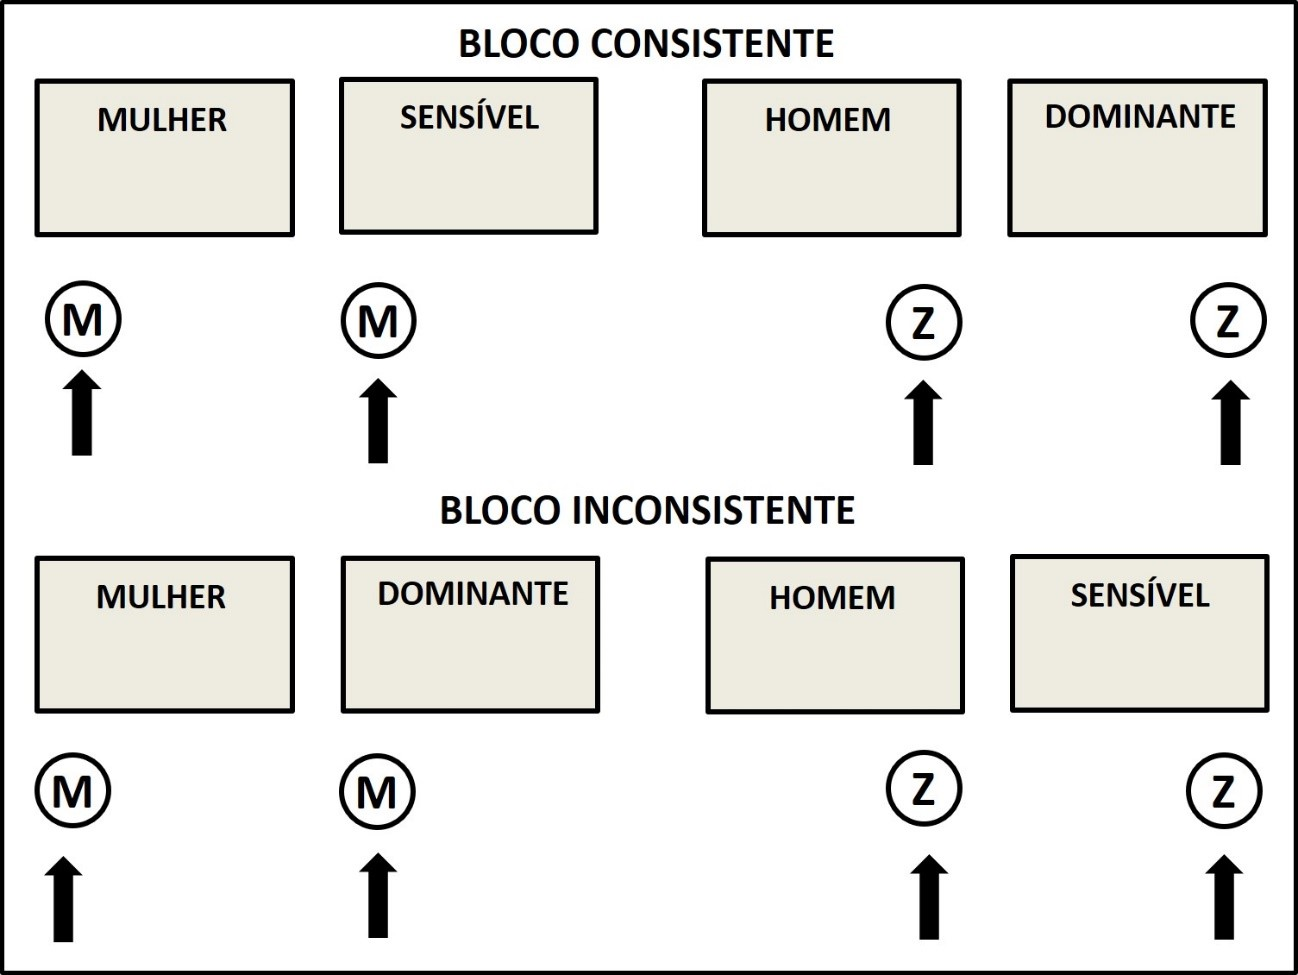
\includegraphics[width=\linewidth]{5/figura3.jpg}
    \caption{Modelo esquemático dos quatro tipos de tentativas hipotéticas do FAST para cada um dos blocos (consistente e inconsistente). Nos blocos de tentativas consistentes (acima) e nos blocos de tentativas inconsistentes (abaixo), a resposta considerada correta é pressionar a mesma tecla do computador, indicada pela seta preta, para cada uma das categorias consideradas corretas naquele bloco.}
    \label{fig3}
\end{figure}

Para verificar a validade do FAST na detecção de relações estereotípicas entre estímulos aprendidas em contexto social, O'Reilly et al. (2012) fizeram um estudo, com 23 participantes, em que relações condicionais entre estímulos abstratos foram ensinadas em ambiente experimental e depois testaram se o FAST seria eficiente em demonstrar a força das relações entre os estímulos relacionados. Em uma das fases experimentais, os participantes eram submetidos a um procedimento de MTS em que aprendiam a relacionar dois pares de estímulos: A1-B1 e A2-B2. As outras três fases eram pares de blocos de tentativas consistentes e inconsistentes com as relações aprendidas usando o procedimento FAST, tanto com os estímulos treinados na fase de MTS quanto com novos estímulos para estabelecer uma linha de base de comparação. Os resultados mostraram que dos 18 participantes que terminaram o estudo, 13 fizeram 10 acertos consecutivos mais rapidamente no bloco consistente que no bloco inconsistente usando as relações treinadas anteriormente, mostrando que o FAST pode ser usado para determinar a existência prévia de relações entre estímulos. Posteriormente, outro estudo (O'Reilly, Roche, Gavin, \& Ruiz, 2013) testou se o FAST era capaz de medir a existência e a força de relações derivadas daquelas ensinadas em laboratório usando o paradigma de equivalência de estímulos (Sidman, 1971). Esse teste é especialmente importante, pois, como os autores apontam, as relações verbais aprendidas nas contingências sociais da comunidade verbal muitas vezes estão em cadeias complexas dentro de classes de estímulos equivalentes. Nesse estudo, 24 participantes passaram por três fases experimentais. Na fase 1, receberam treino de relações condicionais com o procedimento de MTS para estabelecer as relações AB e AC. Na fase 2, foram testadas as relações emergentes que atestam a formação de classes de estímulos equivalentes. A fase 3 consistiu em uma série de apresentações do FAST: usando tanto estímulos relacionados diretamente durante o treino de relações condicionais com o procedimento de MTS, como estímulos cujas relações entre si eram emergentes dentro das classes de estímulos equivalentes formadas. Os resultados mostraram que o FAST é sensível para detectar tanto as relações diretamente treinadas quanto as relações derivadas entre os estímulos das classes de equivalência.

As demonstrações experimentais das variáveis envolvidas no procedimento de FAST com relações estabelecidas em laboratório atestam que este é um procedimento válido e eficiente para medidas de atitudes implícitas consistente com a Análise do Comportamento. Sendo assim, pesquisas aplicadas sobre atitudes explícitas do tipo viés de gênero, preconceito e machismo podem se beneficiar do uso do FAST como medida da força das relações aprendidas socialmente dentro de uma cultura. Por exemplo, um estudo recente (Cartwright, Roche, Gogarty, O'Reilly, \& Stewart, 2016) avaliou, pela primeira vez, a sensibilidade do FAST a relações naturais (não treinadas em laboratório), ao verificar estereótipos de gênero implícitos dos participantes quanto a características estereotipicamente femininas e masculinas. Para isso, os experimentadores selecionaram palavras consideradas tradicionalmente como qualidades masculinas (``dominante'', ``racional'', ``competitivo'' e ``agressivo'') e femininas (``submissa'', ``emocional'', ``cooperativa'' e ``passiva'') e formaram duas categorias consistentes entre um estímulo rótulo (a palavra ``homem'' ou a palavra ``mulher'') e os estímulos de características consideradas masculinas na categoria ``homem'' e os estímulos de características femininas na categoria ``mulher''. Os blocos de tentativas inconsistentes apresentavam os estímulos ``homem'' e características consideradas femininas controlando a mesma resposta e os estímulos ``mulher'' e características masculinas controlando outra resposta. Trinta estudantes universitários foram participantes do estudo. Além dos blocos de FAST, eles também foram submetidos à apresentação do IAT e a dois questionários de autorrelato para a medida da atitude explícita. Os resultados mostraram que o FAST é sensível a relações verbais anteriormente aprendidas entre estímulos – mais especificamente a relações pervasivas de estereótipo de gênero. Todos os 30 participantes mostraram efeitos na direção esperada: aprendizagem mais rápida da resposta comum no bloco de tentativas consistentes do que no bloco de tentativas inconsistentes. Além disso, para os 27 dos 28 participantes que concluíram também o IAT, os resultados mostraram latências mais curtas nas respostas dos blocos de relações consistentes com os estereótipos de gênero. Como esperado pelos pesquisadores, não foram encontradas correlações entre as medidas implícitas e explícitas.

A importância de se ter um teste de medida implícita para se estudar estereótipo de gênero é mais bem compreendida quando pensamos que a desigualdade de gênero é um problema social a nível global, preocupando diversos países no mundo e mobilizando instituições e governos a superá-lo, sendo inclusive uma das metas da Organização das Nações Unidas (ONU, 2015). No Brasil, o Centro de Atendimento à Mulher, que tem um plantão telefônico (180), indicou que entre 2014 e 2015 houve aumento na denúncia de crimes contra mulheres: de 300,39\% nas denúncias de cárcere privado, de 165,27\% nos casos de estupro e de 161,42\% nos relatos de tráfico de pessoas.

Esses dados mostram que o gênero é uma variável relevante na interação verbal entre pessoas. Ruiz (2003) destaca que o gênero é uma fonte tênue de controle de estímulos no comportamento das pessoas, mas que gera contingências muito diferentes para homens e mulheres dentro da sociedade. Nesse estudo, Ruiz (2003) cita diversos exemplos (e.g., Sadker \& Sadker, 1994; Irvine, 1986) de como professores tratam diferentemente meninos e meninas na escola, dando significantemente mais atenção para eles nas aulas e elogiando-os por suas ideias e trabalho enquanto elogiam as meninas pela aparência de seus trabalhos e por elas seguirem regras.

Os estudos experimentais e os diversos procedimentos usados na área de atitudes implícitas demonstram que o aprendizado das relações simbólicas e arbitrárias entre estímulos de naturezas diferentes presentes no ambiente físico ou verbal de um indivíduo, ao longo de sua história dentro de uma cultura, leva a repertórios de comportamentos que se expressam não somente no nível verbal, mas em respostas que agem diretamente sobre o meio físico ou social. As redes de relações entre estímulos estabelecidas pelas práticas culturais tornam virtualmente impossível que analisemos os fenômenos comportamentais humanos sem uma compreensão ampla dos contextos em que essas relações foram aprendidas e quais as funções que elas adquirem no controle do comportamento dos indivíduos dentro do grupo. Para de Rose (2016) 

\begin{quote}
    Isto inclui uma ampla gama de funções, que podem ser agrupadas em discriminativas, eliciadoras e reforçadoras condicionadas. Assim, se um estímulo é discriminativo, eliciador, ou reforçador condicionado, estímulos coordenados a ele podem adquirir estas mesmas funções, mesmo que não tenha havido para eles um treino específico de discriminação operante ou de condicionamento respondente (p. 210).
\end{quote}

Na prática, isso quer dizer que, numa situação social, quando rimos de comentários machistas sobre a roupa de uma mulher, estamos reforçando as relações entre esses estímulos, relações que participam de uma rede complexa de relações com outros estímulos, respostas e reforçadores, que também terão suas probabilidades de ocorrência modificadas. Atitudes implícitas são o produto do controle simbólico sobre o comportamento das pessoas dentro de uma cultura. Para além da descrição das relações entre eventos que controlam as respostas atitudinais implícitas, o uso de procedimentos experimentais que evidenciam a força dessas relações no controle dos comportamentos verbais e não verbais dos indivíduos dentro de uma prática cultural é necessário para que a Análise do Comportamento passe a considerar esses contextos de controle como parte imprescindível em uma análise cultural que se traduza em mudança efetiva de sistemas de opressão.
\vfill
\pagebreak
\section*{Referências Bibliográficas}\sectionmark{Referências Bibliográficas}

\hangindent=25pt
\hangafter=1
\noindent Ajzen, I., \& Madden, T.J. (1986). Prediction of goal-directed behavior-attitudes, intentions, and perceived behavioral-control. \textit{Journal of Experimental Social Psychology, 22}(5), 453-474.

\hangindent=25pt
\hangafter=1
\noindent Barnes, D., \& Keenan, M. (1993). A transfer of functions through derived arbitrary and nonarbitrary stimulus relations. \textit{Journal of the Experimental Analysis of Behavior, 59}(1), 61-81.

\hangindent=25pt
\hangafter=1
\noindent Barnes, D., Browne, M., Smeets, P., \& Roche, B. (1995). A transfer of functions and a conditional transfer of functions through equivalence relations in three-to six-year-old children. \textit{The Psychological Record, 45}(3), 405-430.

\hangindent=25pt
\hangafter=1
\noindent Barnes-Holmes, D., Barnes-Holmes, Y., Power, P., Hayden, E., Milne, R., \& Stewart, I. (2006). Do you really know what you believe? Developing the Implicit Relational Assessment Procedure (IRAP) as a direct measure of implicit beliefs. \textit{The Irish Psychologist, 32}(7), 169-177.

\hangindent=25pt
\hangafter=1
\noindent Barnes-Holmes, D., Barnes-Holmes, Y., Stewart, I., \& Boles, S. (2010). A sketch of the Implicit Relational Assessment Procedure (IRAP) and the relational elaboration and coherence (REC) model. \textit{The Psychological Record, 60}, 527-542.

\hangindent=25pt
\hangafter=1
\noindent Bem, D.J. (1965). An experimental analysis of self-persuasion. \textit{Journal of Experimental Social Psychology, 1}, 199-218.

\hangindent=25pt
\hangafter=1
\noindent Cartwright, A., Roche, B., Gogarty, M., O'Reilly, A., \& Stewart, I. (2016). Using a modified Function Aquisition Speed Test (FAST) for assessing implicit gender stereotypes. \textit{The Psychological Record, 66}, 223-233.

\hangindent=25pt
\hangafter=1
\noindent Cartwright, A., Hussey, I., Roche, B., Dunne, J., \& Murphy, C. (2017). An investigation into the relationship between the gender binary and occupational discrimination using the Implicit Relational Assessment Procedure. \textit{The Psychological Record, 67}(1), 121-130.

\hangindent=25pt
\hangafter=1
\noindent Catania, C.A. (2017). \textit{Prejudice as verbally governed discrimination. The ABCs of Behavior Analysis: Introduction to Behavior and and Learning}, (pp. 254-263). Cornwall-on-Hudson, NY: Sloan Publi\-shing. 

\hangindent=25pt
\hangafter=1
\noindent Crowne, D.P., \& Marlowe, D. (1960). A new scale of social desirability independent of psychopathology. \textit{Journal of Consulting Psychology, 24}(4), 349-354.

\hangindent=25pt
\hangafter=1
\noindent de Rose, J.C. (2016). A importância dos respondentes e das relações simbólicas para uma Análise Comportamental da Cultura. \textit{Acta Comportamentalia, 24}(2), 201-220.

\hangindent=25pt
\hangafter=1
\noindent Drake, C.E., Kellum, K.K., Wilson, K.G., Luoma, J.B., Weinstein, J.H., \& Adams, C.H. (2010). Examining the Implicit Relational Assessment Procedure: Four preliminary studies. \textit{The Psychological Record, 60}(1), 81–100.

\hangindent=25pt
\hangafter=1
\noindent Drake, C.E., Primeaux, S., \& Thomas, J. (2018). Comparing implicit gender stereotypes between women and men with the Implicit Relational Assessment Procedure. \textit{Gender Issues, 35}(1), 3-20.

\hangindent=25pt
\hangafter=1
\noindent Farrell, L., Cochrane, A., \& McHugh, L. (2015). Exploring attitudes to\-wards gender and science: The advantages of an IRAP approach versus the IAT. \textit{Journal of Contextual Behavioral Science, 4}, 121-128.

\hangindent=25pt
\hangafter=1
\noindent Fazio, R.H., \& Olson, M.A. (2003). Implicit measures in social cognition research: Their meaning and use. \textit{Annual Review of Psychology, 54}(1), 297-327.

\hangindent=25pt
\hangafter=1
\noindent Field, D.P., \& Hineline, P.N. (2008). Dispositioning and the obscured roles of time in psychological explanations. \textit{Behavior and Philosophy, 36}, 5-69.

\hangindent=25pt
\hangafter=1
\noindent Freitas, J.C. (2017). \textit{O IRAP como instrumento para identificação de vieses de gênero: uma revisão de literatura}. Apresentação Oral em Sessão Coordenada no XXVI Encontro Brasileiro de Psicologia e Medicina Comportamental. Bauru, SP.

\hangindent=25pt
\hangafter=1
\noindent Gawronski, B., \& Bodenhausen, G.V. (2006). Associative and propositional processesin evaluation: an integrative review of implicit and explicit attitude change. \textit{Psychological Bulletin, 132}(5), 692-731.

\hangindent=25pt
\hangafter=1
\noindent Greenwald, A.G., McGhee, D.E., \& Schwartz, J.L. (1998). Measuring individual differences in implicit cognition: The Implicit Association Test. \textit{Journal of Personality and Social Psychology, 74}, 1464-1480.

\hangindent=25pt
\hangafter=1
\noindent Guerin, B. (1994). Attitudes and beliefs as verbal behavior. \textit{The Behavior Analyst, 17}(1), 155-163.

\hangindent=25pt
\hangafter=1
\noindent Hayes, S.C., Barnes-Holmes, D., \& Roche, B. (2001). \textit{Relational Frame Theory: A post Skinnerian account of human language and cognition.} New York: Plenum Press.

\hangindent=25pt
\hangafter=1
\noindent Hineline, P.N. (1990). The origins of environment-based psychological theory. \textit{Journal of the Experimental Analysis of Behavior, 53}(2), 305-320.

\hangindent=25pt
\hangafter=1
\noindent Holland, J. (1973). ¿Servirán los principios conductuales para los revolucionarios? Em F.S. Keller \& E.R. Iñesta, (Orgs.), \textit{Modificación de la conduta: Aplicaciones a la educación}. México: Trillas.

\hangindent=25pt
\hangafter=1
\noindent Hussey, I., Mhaoileoin, D.N., Barnes-Holmes, D., Ohtsuki, T., Kishita, N., Hughes, S., \& Murphy, C. (2016). The IRAP is nonrelative but not acontextual: Changes to the contrast category influence men’s dehumanization of women. The \textit{Psychological Record, 66}(2), 291-299. 

\hangindent=25pt
\hangafter=1
\noindent Israel, A.C. (1978). Some thoughts on correspondence between saying and doing. \textit{Journal of Applied Behavior Analysis, 11}(2), 271-276.

\hangindent=25pt
\hangafter=1
\noindent Israel, A.C., \& O'Leary, K.D. (1973). Developing correspondence be\-tween children's words and deeds. \textit{Child Development, 14}, 575-581.

\hangindent=25pt
\hangafter=1
\noindent Kashima, Y., Gallois, C., \& McCamish, M. (1993). The theory of reasoned action and cooperative behaviour: It takes two to use a condom. \textit{British Journal of Social Psychology, 32}, 227-239.

\hangindent=25pt
\hangafter=1
\noindent Lloyd, K.E. (1994). Do as I say, not as I do. \textit{The Behavior Analyst, 17}(1), 131-139.

\hangindent=25pt
\hangafter=1
\noindent Maio, G.R., Haddock, G., Manstead, A.S., \& Spears, R. (2010). Attitudes and intergroup relations. Em T.D. Nelson, (Ed.), \textit{Handbook of prejudice, stereotyping, and discrimination}, (pp. 261-275). New York: Psychology Press. 

\hangindent=25pt
\hangafter=1
\noindent Nolan, J., Murphy, C., \& Barnes-Holmes, D. (2013). Implicit relational assessment procedure and body-weight bias: Influence of gender of participants and targets. The \textit{Psychological Record, 63}(3), 467-488.

\hangindent=25pt
\hangafter=1
\noindent Nosek, B.A., Hawkins, C.B., \& Frazier, R.S. (2011). Implicit social cognition: from measures to mechanisms. \textit{Trends in Cognitive Sciences, 15}, 152-159.

\hangindent=25pt
\hangafter=1
\noindent O'Reilly, A., Roche, B., Gavin, A., \& Ruiz, M. R. (2013). A function acquisition speed test for equivalence relations (FASTER). \textit{The Psychological Record, 63}, 707-724.

\hangindent=25pt
\hangafter=1
\noindent O'Reilly, A., Roche, B., Ruiz, M., Tyndall, I., \& Gavin, A. (2012). The function acquisition speed test (FAST): a behavior analytic implicit test for assessing stimulus relations. \textit{The Psychological Record, 62}(3), 507–528.

\hangindent=25pt
\hangafter=1
\noindent Organização das Nações Unidas. (2015). \textit{Minimum Set of Gender Indicators}. Recuperado de: \url{https://genderstats.un.org}.

\hangindent=25pt
\hangafter=1
\noindent Rabelo, L.Z., Bortoloti, R., \& Souza, D.H. (2014). Dolls are for girls and not for boys: Evaluating the appropriateness of the Implicit Relational Assessment Procedure for school-age children. \textit{The Psychological Record, 64}(1), 71-77.

\hangindent=25pt
\hangafter=1
\noindent Ruiz, M. R. (2003). Inconspicuous sources of behavioral control: The case of gendered practices. \textit{The Behavior Analyst Today, 4}(1), 12-16.

\hangindent=25pt
\hangafter=1
\noindent Scanlon, G., McEnteggart, C., Barnes-Holmes, Y., \& Barnes-Holmes, D. (2014). Using the implicit relational assessment procedure (IRAP) to assess implicit gender bias and self-esteem in typically-devel\-oping children and children with ADHD and with dyslexia. \textit{Behavioral Development Bulletin, 19}(2), 48-59.

\hangindent=25pt
\hangafter=1
\noindent Sidman, M. (1960). \textit{Tactics of scientific research}. New York: Basic Books.

\hangindent=25pt
\hangafter=1
\noindent Sidman, M. (1971). Reading and auditory-visual equivalences. \textit{Journal of Speech and Hearing Research, 14}, 5-13.

\hangindent=25pt
\hangafter=1
\noindent Sidman, M. (1994). \textit{Equivalence relations and behavior: A research story}. Boston: Authors Cooperative.

\hangindent=25pt
\hangafter=1
\noindent Sidman, M. (1997). Equivalence relations. \textit{Journal of the Experimental Analysis of Behavior, 68}(2), 258-266.

\hangindent=25pt
\hangafter=1
\noindent Sidman, M., \& Cresson, O. (1973). Reading and crossmodal transfer of stimulus equivalences in severe retardation. \textit{American Journal of Mental Retardation, 77}, 515-523.

\hangindent=25pt
\hangafter=1
\noindent Sidman, M., \& Tailby, W. (1982). Conditional discrimination vs. matching to sample: An expansion of the testing paradigm. \textit{Journal of the Experimental Analysis of Behavior, 37}, 5-22.

\hangindent=25pt
\hangafter=1
\noindent Sidman, M., Rauzin, R., Lazar, R., Cunningham, S., Tailby, W., \& Carrigan, P. (1982). A search for symmetry in the conditional discrimination of rhesus monkeys, baboons, and children. \textit{Journal of the Experimental Analysis of Behavior, 37}, 23-44.

\hangindent=25pt
\hangafter=1
\noindent Skinner, B.F. (1961). Why we need teaching machines. \textit{Harvard Educational Review, 31}, 377-398. 

\hangindent=25pt
\hangafter=1
\noindent Skinner, B. F. (1957). \textit{Verbal Behavior}. Acton, Massachusetts: Copley.

\hangindent=25pt
\hangafter=1
\noindent Skinner, B. F. (1953). \textit{Science and human behavior}. New York: Macmillan. 

\hangindent=25pt
\hangafter=1
\noindent Watt, A., Keenan, M., Barnes, D., \& Cairns, E. (1991). Social categorization and stimulus equivalence. \textit{The Psychological Record, 41}, 33-50.